%%%%%%%%%%%%%%%%%%%%%%%%%%%%%%%%%%%%%%%%%
%  My documentation report
%  Objetive: Explain what I did and how, so someone can continue with the investigation
%
% Important note:
% Chapter heading images should have a 2:1 width:height ratio,
% e.g. 920px width and 460px height.
%
%%%%%%%%%%%%%%%%%%%%%%%%%%%%%%%%%%%%%%%%%


%----------------------------------------------------------------------------------------
%	PACKAGES AND OTHER DOCUMENT CONFIGURATIONS
%----------------------------------------------------------------------------------------

\documentclass[11pt,fleqn]{book} % Default font size and left-justified equations

\usepackage[top=3cm,bottom=3cm,left=3.2cm,right=3.2cm,headsep=10pt,letterpaper]{geometry} % Page margins

\usepackage{xcolor} % Required for specifying colors by name
\definecolor{ocre}{RGB}{52,177,201} % Define the orange color used for highlighting throughout the book%

% Font Settings
\usepackage{avant} % Use the Avantgarde font for headings
%\usepackage{times} % Use the Times font for headings
\usepackage{mathptmx} % Use the Adobe Times Roman as the default text font together with math symbols from the Sym­bol, Chancery and Com­puter Modern fonts
\usepackage{microtype} % Slightly tweak font spacing for aesthetics
\usepackage[utf8]{inputenc} % Required for including letters with accents
\usepackage[T1]{fontenc} % Use 8-bit encoding that has 256 glyphs
\usepackage{amsthm}
%%%

% Bibliography
\usepackage[style=alphabetic,sorting=nyt,sortcites=true,autopunct=true,babel=hyphen,hyperref=true,abbreviate=false,backref=true,backend=biber]{biblatex}
\addbibresource{bibliography.bib} % BibTeX bibliography file
\defbibheading{bibempty}{}

%----------------------------------------------------------------------------------------
%	VARIOUS REQUIRED PACKAGES
%----------------------------------------------------------------------------------------

\usepackage{titlesec} % Allows customization of titles

\usepackage{graphicx} % Required for including pictures
\graphicspath{{Pictures/}} % Specifies the directory where pictures are stored
% \graphicspath{{Plots/}}
\usepackage{lipsum} % Inserts dummy text

\usepackage{tikz} % Required for drawing custom shapes

\usepackage[english]{babel} % English language/hyphenation

\usepackage{enumitem} % Customize lists
\setlist{nolistsep} % Reduce spacing between bullet points and numbered lists

\usepackage{booktabs} % Required for nicer horizontal rules in tables

\usepackage{eso-pic} % Required for specifying an image background in the title page

%----------------------------------------------------------------------------------------
%	MAIN TABLE OF CONTENTS
%----------------------------------------------------------------------------------------

\usepackage{titletoc} % Required for manipulating the table of contents

\contentsmargin{0cm} % Removes the default margin
% Chapter text styling
\titlecontents{chapter}[1.25cm] % Indentation
{\addvspace{15pt}\large\sffamily\bfseries} % Spacing and font options for chapters
{\color{ocre!60}\contentslabel[\Large\thecontentslabel]{1.25cm}\color{ocre}} % Chapter number
{}  
{\color{ocre!60}\normalsize\sffamily\bfseries\;\titlerule*[.5pc]{.}\;\thecontentspage} % Page number
% Section text styling
\titlecontents{section}[1.25cm] % Indentation
{\addvspace{5pt}\sffamily\bfseries} % Spacing and font options for sections
{\contentslabel[\thecontentslabel]{1.25cm}} % Section number
{}
{\sffamily\hfill\color{black}\thecontentspage} % Page number
[]
% Subsection text styling
\titlecontents{subsection}[1.25cm] % Indentation
{\addvspace{1pt}\sffamily\small} % Spacing and font options for subsections
{\contentslabel[\thecontentslabel]{1.25cm}} % Subsection number
{}
{\sffamily\;\titlerule*[.5pc]{.}\;\thecontentspage} % Page number
[] 

%----------------------------------------------------------------------------------------
%	MINI TABLE OF CONTENTS IN CHAPTER HEADS
%----------------------------------------------------------------------------------------

% Section text styling
\titlecontents{lsection}[0em] % Indendating
{\footnotesize\sffamily} % Font settings
{}
{}
{}

% Subsection text styling
\titlecontents{lsubsection}[.5em] % Indentation
{\normalfont\footnotesize\sffamily} % Font settings
{}
{}
{}
 
%----------------------------------------------------------------------------------------
%	PAGE HEADERS
%----------------------------------------------------------------------------------------

\usepackage{fancyhdr} % Required for header and footer configuration

\pagestyle{fancy}
\renewcommand{\chaptermark}[1]{\markboth{\sffamily\normalsize\bfseries\chaptername\ \thechapter.\ #1}{}} % Chapter text font settings
\renewcommand{\sectionmark}[1]{\markright{\sffamily\normalsize\thesection\hspace{5pt}#1}{}} % Section text font settings
\fancyhf{} \fancyhead[LE,RO]{\sffamily\normalsize\thepage} % Font setting for the page number in the header
\fancyhead[LO]{\rightmark} % Print the nearest section name on the left side of odd pages
\fancyhead[RE]{\leftmark} % Print the current chapter name on the right side of even pages
\renewcommand{\headrulewidth}{0.5pt} % Width of the rule under the header
\addtolength{\headheight}{2.5pt} % Increase the spacing around the header slightly
\renewcommand{\footrulewidth}{0pt} % Removes the rule in the footer
\fancypagestyle{plain}{\fancyhead{}\renewcommand{\headrulewidth}{0pt}} % Style for when a plain pagestyle is specified

% Removes the header from odd empty pages at the end of chapters
\makeatletter
\renewcommand{\cleardoublepage}{
\clearpage\ifodd\c@page\else
\hbox{}
\vspace*{\fill}
\thispagestyle{empty}
\newpage
\fi}

%----------------------------------------------------------------------------------------
%	THEOREM STYLES
%----------------------------------------------------------------------------------------

\usepackage{amsmath,amsfonts,amssymb,amsthm} % For math equations, theorems, symbols, etc

\newcommand{\intoo}[2]{\mathopen{]}#1\,;#2\mathclose{[}}
\newcommand{\ud}{\mathop{\mathrm{{}d}}\mathopen{}}
\newcommand{\intff}[2]{\mathopen{[}#1\,;#2\mathclose{]}}
\newtheorem{notation}{Notation}[chapter]

%%%%%%%%%%%%%%%%%%%%%%%%%%%%%%%%%%%%%%%%%%%%%%%%%%%%%%%%%%%%%%%%%%%%%%%%%%%
%%%%%%%%%%%%%%%%%%%% dedicated to boxed/framed environements %%%%%%%%%%%%%%
%%%%%%%%%%%%%%%%%%%%%%%%%%%%%%%%%%%%%%%%%%%%%%%%%%%%%%%%%%%%%%%%%%%%%%%%%%%
\newtheoremstyle{ocrenumbox}% % Theorem style name
{0pt}% Space above
{0pt}% Space below
{\normalfont}% % Body font
{}% Indent amount
{\small\bf\sffamily\color{ocre}}% % Theorem head font
{\;}% Punctuation after theorem head
{0.25em}% Space after theorem head
{\small\sffamily\color{ocre}\thmname{#1}\nobreakspace\thmnumber{\@ifnotempty{#1}{}\@upn{#2}}% Theorem text (e.g. Theorem 2.1)
\thmnote{\nobreakspace\the\thm@notefont\sffamily\bfseries\color{black}---\nobreakspace#3.}} % Optional theorem note
\renewcommand{\qedsymbol}{$\blacksquare$}% Optional qed square

\newtheoremstyle{blacknumex}% Theorem style name
{5pt}% Space above
{5pt}% Space below
{\normalfont}% Body font
{} % Indent amount
{\small\bf\sffamily}% Theorem head font
{\;}% Punctuation after theorem head
{0.25em}% Space after theorem head
{\small\sffamily{\tiny\ensuremath{\blacksquare}}\nobreakspace\thmname{#1}\nobreakspace\thmnumber{\@ifnotempty{#1}{}\@upn{#2}}% Theorem text (e.g. Theorem 2.1)
\thmnote{\nobreakspace\the\thm@notefont\sffamily\bfseries---\nobreakspace#3.}}% Optional theorem note

\newtheoremstyle{blacknumbox} % Theorem style name
{0pt}% Space above
{0pt}% Space below
{\normalfont}% Body font
{}% Indent amount
{\small\bf\sffamily}% Theorem head font
{\;}% Punctuation after theorem head
{0.25em}% Space after theorem head
{\small\sffamily\thmname{#1}\nobreakspace\thmnumber{\@ifnotempty{#1}{}\@upn{#2}}% Theorem text (e.g. Theorem 2.1)
\thmnote{\nobreakspace\the\thm@notefont\sffamily\bfseries---\nobreakspace#3.}}% Optional theorem note

%%%%%%%%%%%%%%%%%%%%%%%%%%%%%%%%%%%%%%%%%%%%%%%%%%%%%%%%%%%%%%%%%%%%%%%%%%%
%%%%%%%%%%%%% dedicated to non-boxed/non-framed environements %%%%%%%%%%%%%
%%%%%%%%%%%%%%%%%%%%%%%%%%%%%%%%%%%%%%%%%%%%%%%%%%%%%%%%%%%%%%%%%%%%%%%%%%%
\newtheoremstyle{ocrenum}% % Theorem style name
{5pt}% Space above
{5pt}% Space below
{\normalfont}% % Body font
{}% Indent amount
{\small\bf\sffamily\color{ocre}}% % Theorem head font
{\;}% Punctuation after theorem head
{0.25em}% Space after theorem head
{\small\sffamily\color{ocre}\thmname{#1}\nobreakspace\thmnumber{\@ifnotempty{#1}{}\@upn{#2}}% Theorem text (e.g. Theorem 2.1)
\thmnote{\nobreakspace\the\thm@notefont\sffamily\bfseries\color{black}---\nobreakspace#3.}} % Optional theorem note
\renewcommand{\qedsymbol}{$\blacksquare$}% Optional qed square
\makeatother

% Defines the theorem text style for each type of theorem to one of the three styles above
\newcounter{dummy} 
\numberwithin{dummy}{section}
\theoremstyle{ocrenumbox}


\newtheorem{theoremeT}[dummy]{Theorem}
\newtheorem{lemma}[dummy]{Lemma}
\newtheorem{observation}[dummy]{Observation}
\newtheorem{proposition}[dummy]{Proposition}
% \newtheorem{definition}[dummy]{Definition}
\newtheorem{claim}[dummy]{Claim}
\newtheorem{fact}[dummy]{Fact}
\newtheorem{assumption}[dummy]{Assumption}

\newtheorem{problem}{Problem}[chapter]
% \newtheorem{exercise}{Exercise}[chapter]
\theoremstyle{blacknumex}
\newtheorem{exampleT}{Example}[chapter]
\theoremstyle{blacknumbox}
\newtheorem{vocabulary}{Vocabulary}[chapter]
\newtheorem{definitionT}{Definition}[section]
\newtheorem{corollaryT}[dummy]{Corollary}
\theoremstyle{ocrenum}

%----------------------------------------------------------------------------------------
%	DEFINITION OF COLORED BOXES
%----------------------------------------------------------------------------------------

\RequirePackage[framemethod=default]{mdframed} % Required for creating the theorem, definition, exercise and corollary boxes

% Theorem box
\newmdenv[skipabove=7pt,
skipbelow=7pt,
backgroundcolor=black!5,
linecolor=ocre,
innerleftmargin=5pt,
innerrightmargin=5pt,
innertopmargin=5pt,
leftmargin=0cm,
rightmargin=0cm,
innerbottommargin=5pt]{tBox}

% Exercise box	  
\newmdenv[skipabove=7pt,
skipbelow=7pt,
rightline=false,
leftline=true,
topline=false,
bottomline=false,
backgroundcolor=ocre!10,
linecolor=ocre,
innerleftmargin=5pt,
innerrightmargin=5pt,
innertopmargin=5pt,
innerbottommargin=5pt,
leftmargin=0cm,
rightmargin=0cm,
linewidth=4pt]{eBox}	

% Definition box
\newmdenv[skipabove=7pt,
skipbelow=7pt,
rightline=false,
leftline=true,
topline=false,
bottomline=false,
linecolor=ocre,
innerleftmargin=5pt,
innerrightmargin=5pt,
innertopmargin=0pt,
leftmargin=0cm,
rightmargin=0cm,
linewidth=4pt,
innerbottommargin=0pt]{dBox}	

% Corollary box
\newmdenv[skipabove=7pt,
skipbelow=7pt,
rightline=false,
leftline=true,
topline=false,
bottomline=false,
linecolor=gray,
backgroundcolor=black!5,
innerleftmargin=5pt,
innerrightmargin=5pt,
innertopmargin=5pt,
leftmargin=0cm,
rightmargin=0cm,
linewidth=4pt,
innerbottommargin=5pt]{cBox}

% Creates an environment for each type of theorem and assigns it a theorem text style from the "Theorem Styles" section above and a colored box from above
\newenvironment{theorem}{\begin{tBox}\begin{theoremeT}}{\end{theoremeT}\end{tBox}}
\newenvironment{exercise}{\begin{eBox}\begin{exerciseT}}{\hfill{\color{ocre}\tiny\ensuremath{\blacksquare}}\end{exerciseT}\end{eBox}}				  
\newenvironment{definition}{\begin{dBox}\begin{definitionT}}{\end{definitionT}\end{dBox}}	
\newenvironment{example}{\begin{exampleT}}{\hfill{\tiny\ensuremath{\blacksquare}}\end{exampleT}}		
\newenvironment{corollary}{\begin{cBox}\begin{corollaryT}}{\end{corollaryT}\end{cBox}}
\newtheorem{solution}{Solution}[chapter]
\newtheorem{exerciseT}{Exercise}[chapter]

%----------------------------------------------------------------------------------------
%	REMARK ENVIRONMENT
%----------------------------------------------------------------------------------------

\newenvironment{remark}{\par\vspace{10pt}\small % Vertical white space above the remark and smaller font size
\begin{list}{}{
\leftmargin=35pt % Indentation on the left
\rightmargin=25pt}\item\ignorespaces % Indentation on the right
\makebox[-2.5pt]{\begin{tikzpicture}[overlay]
\node[draw=ocre!60,line width=1pt,circle,fill=ocre!25,font=\sffamily\bfseries,inner sep=2pt,outer sep=0pt] at (-15pt,0pt){\textcolor{ocre}{R}};\end{tikzpicture}} % Orange R in a circle
\advance\baselineskip -1pt}{\end{list}\vskip5pt} % Tighter line spacing and white space after remark

%----------------------------------------------------------------------------------------
%	SECTION NUMBERING IN THE MARGIN
%----------------------------------------------------------------------------------------

\makeatletter
\renewcommand{\@seccntformat}[1]{\llap{\textcolor{ocre}{\csname the#1\endcsname}\hspace{1em}}}                    
\renewcommand{\section}{\@startsection{section}{1}{\z@}
{-4ex \@plus -1ex \@minus -.4ex}
{1ex \@plus.2ex }
{\normalfont\large\sffamily\bfseries}}
\renewcommand{\subsection}{\@startsection {subsection}{2}{\z@}
{-3ex \@plus -0.1ex \@minus -.4ex}
{0.5ex \@plus.2ex }
{\normalfont\sffamily\bfseries}}
\renewcommand{\subsubsection}{\@startsection {subsubsection}{3}{\z@}
{-2ex \@plus -0.1ex \@minus -.2ex}
{.2ex \@plus.2ex }
{\normalfont\small\sffamily\bfseries}}                        
\renewcommand\paragraph{\@startsection{paragraph}{4}{\z@}
{-2ex \@plus-.2ex \@minus .2ex}
{.1ex}
{\normalfont\small\sffamily\bfseries}}

%----------------------------------------------------------------------------------------
%	HYPERLINKS IN THE DOCUMENTS
%----------------------------------------------------------------------------------------

% For an unclear reason, the package should be loaded now and not later
\usepackage{hyperref}
\hypersetup{hidelinks,backref=true,pagebackref=true,hyperindex=true,colorlinks=false,breaklinks=true,urlcolor= ocre,bookmarks=true,bookmarksopen=false,pdftitle={Title},pdfauthor={Author}}

%----------------------------------------------------------------------------------------
%	CHAPTER HEADINGS
%----------------------------------------------------------------------------------------

% The set-up below should be (sadly) manually adapted to the overall margin page septup controlled by the geometry package loaded in the main.tex document. It is possible to implement below the dimensions used in the goemetry package (top,bottom,left,right)... TO BE DONE

\newcommand{\thechapterimage}{}
\newcommand{\chapterimage}[1]{\renewcommand{\thechapterimage}{#1}}

% Numbered chapters with mini tableofcontents
\def\thechapter{\arabic{chapter}}
\def\@makechapterhead#1{
\thispagestyle{empty}
{\centering \normalfont\sffamily
\ifnum \c@secnumdepth >\m@ne
\if@mainmatter
\startcontents
\begin{tikzpicture}[remember picture,overlay]
\node at (current page.north west)
{\begin{tikzpicture}[remember picture,overlay]
\node[anchor=north west,inner sep=0pt] at (0,0) {\includegraphics[width=\paperwidth]{\thechapterimage}};
%%%%%%%%%%%%%%%%%%%%%%%%%%%%%%%%%%%%%%%%%%%%%%%%%%%%%%%%%%%%%%%%%%%%%%%%%%%%%%%%%%%%%
% Commenting the 3 lines below removes the small contents box in the chapter heading
%\fill[color=ocre!10!white,opacity=.6] (1cm,0) rectangle (8cm,-7cm);
%\node[anchor=north west] at (1.1cm,.35cm) {\parbox[t][8cm][t]{6.5cm}{\huge\bfseries\flushleft \printcontents{l}{1}{\setcounter{tocdepth}{2}}}};
\draw[anchor=west] (5cm,-9cm) node [rounded corners=20pt,fill=ocre!10!white,text opacity=1,draw=ocre,draw opacity=1,line width=1.5pt,fill opacity=.6,inner sep=12pt]{\huge\sffamily\bfseries\textcolor{black}{\thechapter. #1\strut\makebox[22cm]{}}};
%%%%%%%%%%%%%%%%%%%%%%%%%%%%%%%%%%%%%%%%%%%%%%%%%%%%%%%%%%%%%%%%%%%%%%%%%%%%%%%%%%%%%
\end{tikzpicture}};
\end{tikzpicture}}
\par\vspace*{230\p@}
\fi
\fi}

% Unnumbered chapters without mini tableofcontents (could be added though) 
\def\@makeschapterhead#1{
\thispagestyle{empty}
{\centering \normalfont\sffamily
\ifnum \c@secnumdepth >\m@ne
\if@mainmatter
\begin{tikzpicture}[remember picture,overlay]
\node at (current page.north west)
{\begin{tikzpicture}[remember picture,overlay]
\node[anchor=north west,inner sep=0pt] at (0,0) {\includegraphics[width=\paperwidth]{\thechapterimage}};
\draw[anchor=west] (5cm,-9cm) node [rounded corners=20pt,fill=ocre!10!white,fill opacity=.6,inner sep=12pt,text opacity=1,draw=ocre,draw opacity=1,line width=1.5pt]{\huge\sffamily\bfseries\textcolor{black}{#1\strut\makebox[22cm]{}}};
\end{tikzpicture}};
\end{tikzpicture}}
\par\vspace*{230\p@}
\fi
\fi
}
\makeatother

%----------------------------------------------------------------------------------------
%	LANGUAGE STYLE
%----------------------------------------------------------------------------------------

\usepackage{xcolor} % Required for specifying colors by name
\definecolor{ocre}{RGB}{243,102,25}
\definecolor{deepblue}{rgb}{0,0,0.5}
\definecolor{deepred}{rgb}{0.6,0,0}
\definecolor{deepgreen}{rgb}{0,0.5,0}

% Default fixed font does not support bold face
\DeclareFixedFont{\ttb}{T1}{txtt}{bx}{n}{12} % for bold
\DeclareFixedFont{\ttm}{T1}{txtt}{m}{n}{12}  % for normal
% Python environment
\usepackage{listings}
% Python style for highlighting
\newcommand\pythonstyle{\lstset{
language=Python,
basicstyle=\ttm,
otherkeywords={self},             % Add keywords here
keywordstyle=\ttb\color{deepblue},
emph={MyClass,__init__},          % Custom highlighting
emphstyle=\ttb\color{deepred},    % Custom highlighting style
stringstyle=\color{deepgreen},
frame=tb,                         % Any extra options here
showstringspaces=false            % 
}}

% Python environment
\lstnewenvironment{python}[1][]
{
\pythonstyle
\lstset{#1}
}
{}

% Python for external files
\newcommand\pythonexternal[2][]{{
\pythonstyle
\lstinputlisting[#1]{#2}}}

% Python for inline
\newcommand\pythoninline[1]{{\pythonstyle\lstinline!#1!}}
%%

 % Insert the commands.tex file which contains the majority of the structure behind the template

%----------------------------------------------------------------------------------------
%	Definitions of new commands
%----------------------------------------------------------------------------------------

\def\R{\mathbb{R}}
\newcommand{\cvx}{convex}
\begin{document}

%----------------------------------------------------------------------------------------
%	TITLE PAGE
%----------------------------------------------------------------------------------------

\begingroup
\thispagestyle{empty}
\AddToShipoutPicture*{\put(0,0){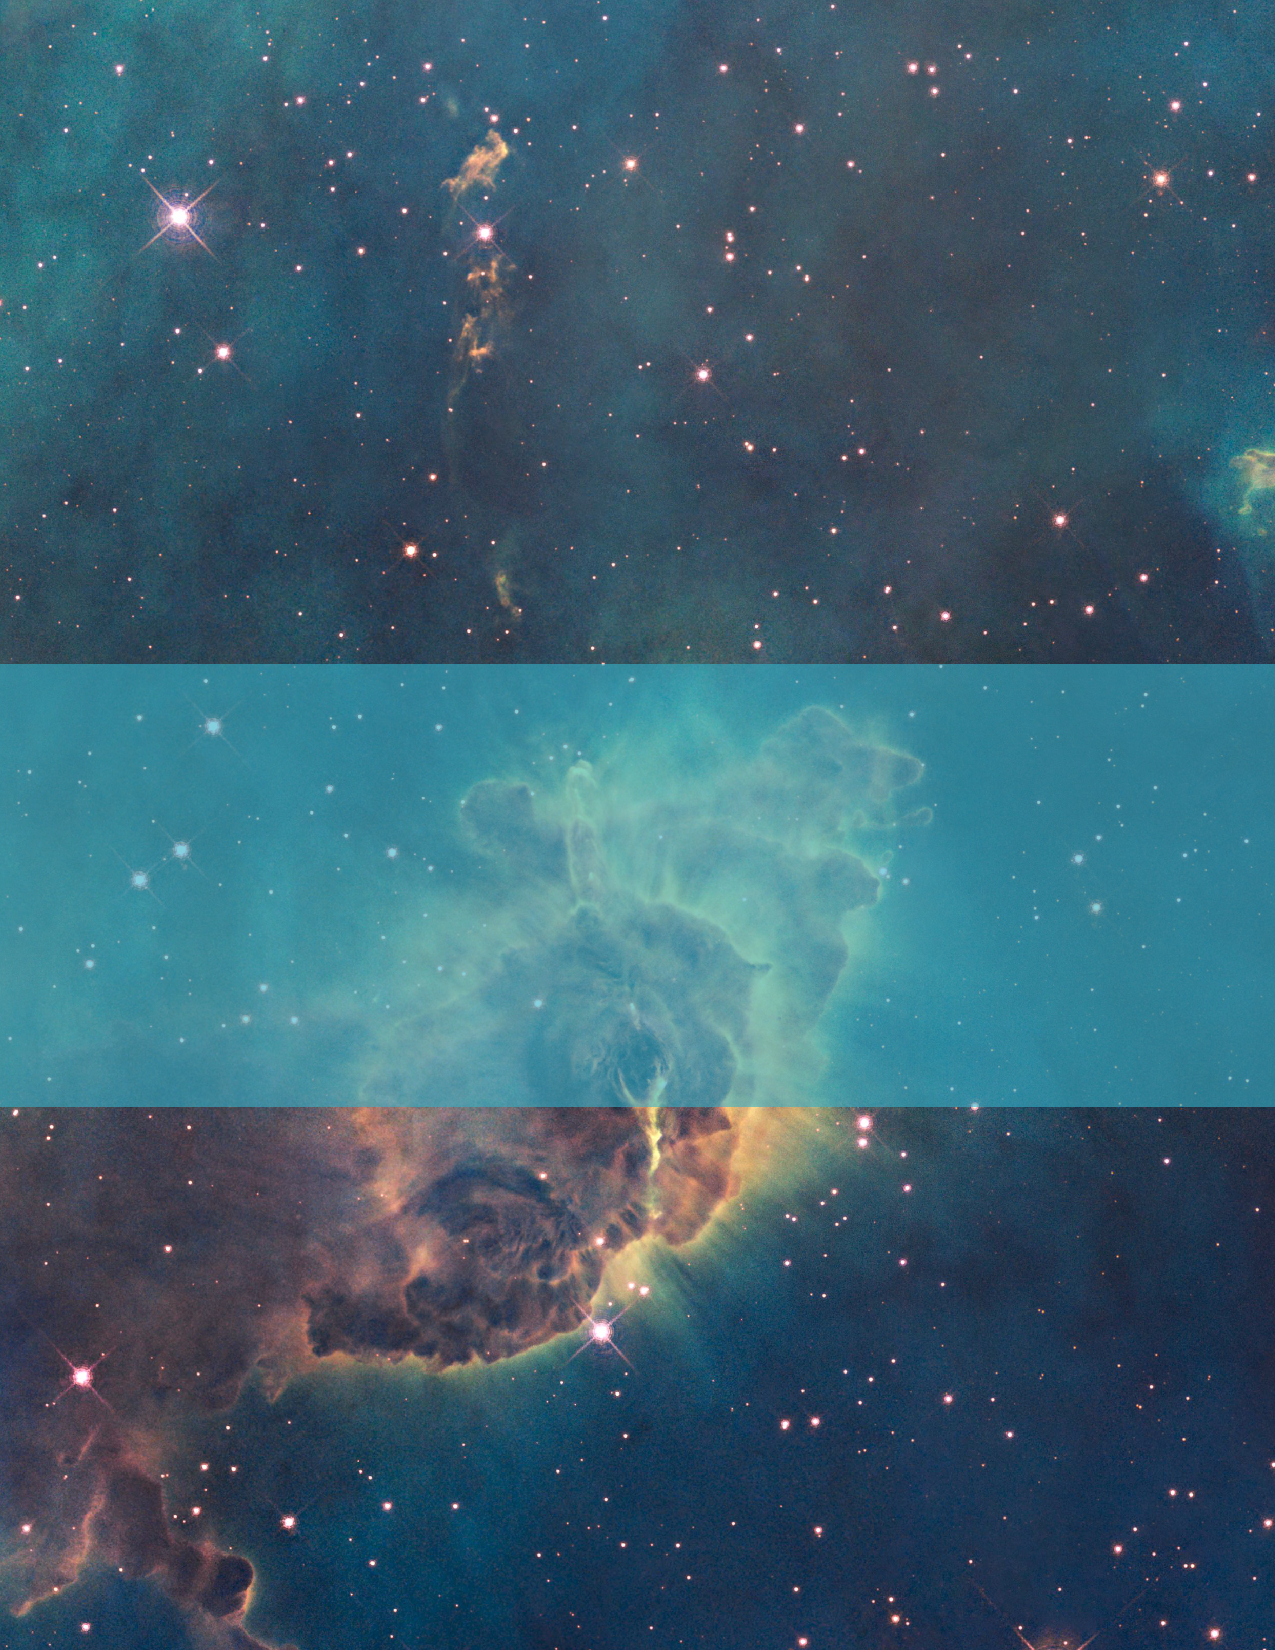
\includegraphics[scale=1.25]{esahubble}}} % Image background
\centering
\vspace*{5cm}
\par\normalfont\fontsize{35}{35}\sffamily\selectfont
\textbf{SymPy par la pratique}\\
{\LARGE Exemple et exercice}\par % Book title
\vspace*{1cm}
{\Huge K.I.A Derouiche}\par % Author name
\endgroup

%----------------------------------------------------------------------------------------
%	COPYRIGHT PAGE
%----------------------------------------------------------------------------------------

\newpage
~\vfill
\thispagestyle{empty}

%\noindent Copyright \copyright\ 2014 Andrea Hidalgo\\ % Copyright notice

\noindent \textsc{Summer Research Internship, University of Western Ontario}\\

\noindent \textsc{github.com/LaurethTeX/Clustering}\\ % URL

\noindent This research was done under the supervision of Dr. Pauline Barmby with the financial support of the MITACS Globalink Research Internship Award within a total of 12 weeks, from June 16th to September 5th of 2014.\\ % License information

\noindent \textit{First release, August 2014} % Printing/edition date

%----------------------------------------------------------------------------------------
%	TABLE OF CONTENTS
%----------------------------------------------------------------------------------------

\chapterimage{head1.png} % Table of contents heading image

\pagestyle{empty} % No headers

\tableofcontents % Print the table of contents itself

%\cleardoublepage % Forces the first chapter to start on an odd page so it's on the right

\pagestyle{fancy} % Print headers again

%----------------------------------------------------------------------------------------
%	AVANT PROPOS
%----------------------------------------------------------------------------------------

\section{Avant-Propos}
Ce livre traite de SymPy, une bibliothèque de calcul symbolique entièrement écrite en Python un langage 
de programmation de haut niveau, orienté objet, totalement libre, conçu pour produire 
du code de qualité, portable et facile à intégrer. Ainsi la conception d'un programme scientifique  ou 
symbolique avec SymPy et Python est très rapide et offre au développeur une bonne productivité. En tant 
que bibliothèque pythonienne elle repose sur un langage dynamique, très souple d'utilisation et 
constitue un complément idéal à des langages compilés. Elle reste une bibliothèque complète et autosuffisant, pour des petits scripts fonctionnels de quelques lignes, comme pour des applicatifs complexes de plusieurs centaines de modules.

\subsection*{Pourquoi ce livre ?}
Il n'existe pas beaucoup d'ouvrages qui traitent du calcul symbolique en générale par  
rapport aux calculs numériques ou des ouvrages consacré aux bibliothèques symbolique écrite en Python 
est en particulier gravitent autour de SymPy mis à part un livre de 50 pages, quelques chapitres ou des 
lignes de codes cité à titre d'exemples. Citons le livre de référence de Svein Linge et Hans Petter 
Langtangen Programming for Computations – Python A Gentle Introduction to Numerical Simulations with 
Python, aux éditions Springer, ou encore une version du livre de 50 pages Instant SymPy Starter de Ronan 
Lamy, aux éditions Packt Publishing Limited, Le livre est Instant SymPy Starter de Ronan Lamy, c'est un 
guide de démarrage rapide, La documentation en ligne de SymPy est bonne, mais il serait plus facile de 
commencer avec ce livre. Alors, pourquoi ce livre ?

Si ce livre présente comme celui de Ronan Lamy les notions de la bibliothèque, celui-la ajoute des  
exemples originaux, des choix dans la présentation des classes, et une approche globale particulière et 
détaillé, il tente également d’ajouter à ce socle des éléments qui participent de la philosophie de la 
programmation en Python scientifique, aller plus loin dans le développement non scientifique, mettre en 
valeur L’Intérêt et l'importance, à savoir :
\begin{itemize}
 \item des conventions de codage ;
 \item combiné l'approche symbolique et numérique;
 \item des bonnes pratiques de programmation et des techniques d’optimisation ;
\end{itemize}

Même si chacun de ces sujets pourrait à lui seul donner matière à des ouvrages entiers, les réunir dans 
un seul et même livre contribue à fournir une vue complète de ce qu’un développeur d'application 
scientifique en particulier et Python averti et son chef de projet mettent en œuvre quotidiennement.

\subsection*{A qui s'adresse l'ouvrage?}
Cet ouvrage s’adresse bien sûr aux développeurs de tous horizons mais également aux
étudiants,chercheurs, enseignants et chefs de projets. Ils ne trouveront pas dans ce livre de bases de 
programmation; une pratique minimale préalable est indispensable de Python, quel que soit le langage 
utilisé. Il n’est pour autant pas nécessaire de maîtriser la programmation orientée objet et 
la connaissance d’un langage impératif est suffisante.
Les développeurs Python débutants – ou les développeurs avertis ne connaissant pas
encore cette bibliothèque – trouveront dans cet ouvrage des techniques et sujets avancées, les patterns 
efficaces et l’application de certains design patterns objet, topologie, théorie des catégories, machine
learning.
Les étudiants et enseignants trouveront un ouvrage ouvert sur l'apprentissage par l'exercice résolus et 
une interprétation d’exercices mathématiques  
les chercheurs trouveront un outil léger et efficace à travers des approches poussées liées aux 
questions récentes en connections avec les mathématiques pures et appliquées de physique théorique.
Les chefs de projets trouveront des éléments pratiques pour augmenter l’efficacité de
leurs équipes pluridisciplinaires, notamment la présentation des principaux modules à la fois issues de  la bibliothèque standard, graphique et numérique.

%----------------------------------------------------------------------------------------
%	CHAPTER 1
%----------------------------------------------------------------------------------------

\chapterimage{head2.png} % Chapter heading image
\section{Introduction}
Ce recueil d'exercices et de problèmes de programmation s'adresse aussi bien aux débutants qu'aux programmeurs confirmés. Il présente en effet plusieurs états d'esprit dont les deux principaux sont la programmation classique en Pascal pour les étudiants du premier cycle universitaire, et la programmation fonctionnelle en Lisp pour le second cycle.

Ce livre constitue un panorama (non exhaustif, mais suffisant) sur les langages de programmation, et offre une grande variété dans les sujets traités : graphiques, calcul matriciel, traitements de chaînes de caractères, graphes, intelligence artificielle...
\\
La première partie du livre sera consacré \`a la résolution par une approche symbolique au divers questions posées au étudiants et toute personnes qui aiment savoir et voir s'initier  pour des niveaux et des questions rencontrés, la deuxième partie du livre sera questions aux problèmes plus rencontrés pour des étudiants passionnée des questions entre mathématiques et technologies, chercheurs et développeurs d'applications scientifiques, la troisième partie plus consacré aux questions poussées  


\subsection{Pourquoi programmer en symbolique }


%----------------------------------------------------------------------------------------
%	CHAPTER 1
%----------------------------------------------------------------------------------------


\chapter{Calcul formel}

L'approche La simulation numérique est devenue essentielle dans de nombreux domaines tels que la mécanique des fluides et des solides, la météo, l'évolution du climat, la biologie ou les semi-conducteurs. Elle permet de comprendre, de prévoir, d'accéder là où les instruments de mesures s'arrêtent. 

Ce livre présente des méthodes performantes du calcul scientifique : matrices creuses, résolution efficace des grands systèmes linéaires, ainsi que de nombreuses applications à la résolution par éléments finis et différences finies. Alternant algorithmes et applications, les programmes sont directement présentés en langage C++. Ils sont sous forme concise et claire, et utilisent largement les notions de classe et de généricité du langage C++. 

Le contenu de ce livre a fait l'objet de cours de troisième année à l'école nationale supérieure d'informatique et de mathématiques appliquées de Grenoble (ENSIMAG) ainsi qu'au mastère de mathématiques appliquées de l'université Joseph Fourier. Des connaissances de base d'algèbre matricielle et de programmation sont recommandées. La maîtrise du contenu de cet ouvrage permet d'appréhender les principaux paradigmes de programmation du calcul scientifique. Il est alors possible d'appliquer ces paradigmes pour aborder des problèmes d'intérêt pratique, tels que la résolution des équations aux dérivées partielles, qui est abordée au cours de ce livre. La diversité des sujets abordés, l'efficacité des algorithmes présentés et leur écriture directe en langage C++ font de cet ouvrage un recueil fort utile dans la vie professionnelle d'un ingénieur. 

Le premier chapitre présente les bases fondamentales pour la suite : présentation du langage C++ à travers la conception d'une classe de quaternions et outils d'analyse asymptotique du temps de calcul des algorithmes. Le second chapitre aborde l'algorithme de transformée de Fourier rapide et développe deux applications à la discrétisation d'équations aux dérivées partielles par la méthode des différences finies. Le troisième chapitre est dédié aux matrices creuses et à l'algorithme du gradient conjugué. Ces notions sont appliquées à la méthode des éléments finis. En annexe sont groupés des exemples de génération de maillage et de visualisation graphique. 

S'il est cependant recommandé de maîtriser les notions du premier chapitre pour aborder le reste du livre, les chapitres deux et trois sont complètement indépendants et peuvent être abordés séparément. Ces chapitres sont complétés par des exercices qui en constituent des développements, ainsi que des notes bibliographiques retraçant l'historique des travaux et fournissant des références sur des logiciels et librairies récents implémentant ou étendant les algorithmes présentés. 

\section{Système de calcul formel}
Dans cette section en va exposer les systèmes de calcul formel, leur 
intérêt qui à vue un renouveau ces dernières années à cause de 
l'émergence de technique, technologie et nouvelle approche de 
programmation pour le domaine scientifique et industriel, hormis le fait 
que le logiciel de calcul formel en soient sont un outil pédagogique 
indispensable pour les scientifiques et les ingénieurs

\begin{example}
Let $G=\{x\in\mathbb{R}^2:|x|<3\}$ and denoted by: $x^0=(1,1)$; consider the function:
\begin{equation}
f(x)=\left\{\begin{aligned} & \mathrm{e}^{|x|} & & \text{si $|x-x^0|\leq 1/2$}\\
& 0 & & \text{si $|x-x^0|> 1/2$}\end{aligned}\right.
\end{equation}
The function $f$ has bounded support, we can take $A=\{x\in\mathbb{R}^2:|x-x^0|\leq 1/2+\epsilon\}$ for all $\epsilon\in\intoo{0}{5/2-\sqrt{2}}$.
\end{example}

qui exprime ce qui nous permet notre choix pour un CAS qui possède des caractéristiques techniques et sur le plan du coût très important quand peut résumer dans les points suivants:
\begin{enumerate}
	\item Leger et 
	\item S’appuie sur le langage de programmation Python
	\item Portabilité dans toute transparence
\end{enumerate}

L'un des systèmes qui peut nous permettre d'écrire cette exemple avec un ordinateurs avec SymPy qui semble mieu intégré

\section{Bibliothèque SymPy}

Dans un cas plus simple l'exemple 1.1 se formule beaucoup plus dans un outil comme SymPy est une bibliothèque de calcul formel elle est aussi un environnement pour 
l’apprentissage de l’algèbre, l’analyse, géométrie, combinatoire, cryptographie, mécanique 
classique et quantique pour le lycée et l’université mais aussi un environnement de 
développement et de recherche. SymPy  écrit entièrement en Python un langage de 
programmation facile à apprendre et adapté à l’apprentissage,  elle fourni aux étudiant 
\textit{SymPyGamma} une application web   notamment des primitives générales de traitement des expressions algébriques (développement, factorisation, …), des aides à l’organisation des objets mathématiques intervenant dans la résolution d’un problème ainsi qu’une assistance à la preuve. Il permet au professeur de préparer et de suivre le travail de l’élève. Différentes maquettes ont été développées et testées auprès d’élèves. Dans la plus récente, nous nous sommes attachés à explorer une nouvelle forme d’activité algébrique. Alors que le calcul en papier crayon et les logiciels standards considèrent
 les expressions de façon isolée, l’environnement que nous développons organise en réseau les différentes expressions intervenant dans la résolution d’un problème. L’ordinateur peut facilement mettre à jour ce réseau quand l’utilisateur modifie certains de ses éléments. Il devient ainsi possible, pour aborder un problème générique, d’explorer facilement des cas particuliers et de conduire une généralisation. Les relations entre expressions algébriques sont mieux mises en évidence du fait de leur invariance dans les modifications du réseau. De façon très concise, Casyopée peut être défini
\subsection{SymPyGamma}
Est une interface onWeb marche avec un navigateur contient plusieurs catégorie liée de calcul, dynamique. L'interet de cette outil qu'il est facilement partageable adapté pour l’enseignement et surtout l'auto-apprentissage 
\subsection{Besoin de rester dans le symbolique}
Le symbolique est une grande importance d'un point de vue technique, car il permet
de limité les risques de bug dans l'exécution des programmes, dans le contexte de 
la vérification formelle si en prend le programme suivant:

\subsection{Passage du symbolique au numérique}
Généralement, le symbolique parmis c'est  
\subsection{Faire des dessins}

%--------------------------------------------------------------------------------------
% CHAPTRE
%--------------------------------------------------------------------------------------

\chapter{Ensemble}

\section{Ensemble}

\subsection{Ensembles}
La notion d'objet immuable en Python est fondamentale,  une structure qui rappel les ensembles en mathématiques que soit fini ou infini est \textit{set}, importante, bien que
dans le cadre de SymPy elle s'appui entièrement sur Python avec certain modification, avec la collection d'objet.
\\

\textit{La fonction set accepte donc en argument un objet de type quelconque et s'efforce de le traduire dans un ensemble. Lorsqu'on ne passe aucun argument à set (option 2), ou qu'on lui passe une liste vide, set renvoie naturellement un ensemble vide; on aurait pu utiliser aussi bien, de la même manière, set(()), set({}), ou même set('') pour arriver au même résultat.}

%\begin{exercise}
%		Définir deux ensembles $X = \lbrace a, b, c, d\rbrace$ et  $Y = \lbrace s, b, d\rbrace$ , puis 			affichez les résultats suivants :
% 		\begin{enumerate}
%  			 \item les ensembles initiaux.
%  			 \item le test d’appartenance de l’élément $c$ à $X$.
%  			 \item le test d’appartenance de l’élément $a$ à $Y$.
%  			 \item les ensembles $X - Y$ et $Y - X$.
%  			 \item l’ensemble $X \cup Y$ (union).
%  			 \item l'ensemble $X \cap Y$ (intersection).
%	 \end{enumerate}
%\end{exercise}

\begin{solution}
Il faut noter qu'il existe une solution qui se base sur le Python builtuints en utilisant la structure de donnée \textit{sets}. Mais comme en n'est dans la logique en utilise 
\begin{python}
from sympy import FiniteSet

X = FiniteSet('a', 'b', 'c', 'd')
Y = FiniteSet('s', 'b', 'd')

class MyClass(Yourclass):
    def __init__(self, my, yours):
        bla = '5 1 2 3 4'
        print bla
\end{python}
\begin{python}
class MyClass(Yourclass):
    def __init__(self, my, yours):
        bla = '5 1 2 3 4'
        print bla
\end{python}

\end{solution}

\chapter{Convex Sets}
\section{Convexity}
\subsection{Cone}
\begin{definition}[Cone]
A set $K \in \R^n$, when $x \in K $ implies $\alpha x \in K$.
\end{definition}
A non convex cone can be hyper-plane.\\
For convex cone $x + y \in K, \forall x,y \in K$.\\
Cone don't need to be "pointed". e.g. \\
Direct sums of cones $C_1 + C_2 = \{ x = x_1+x_2 | x_1 \in C_1, x_2 \in C_2 \}$.\\
\begin{example}
$S_1^n  \{ X | X=X^n ,\lambda(x) \ge 0\}$\\
A matrix with positive eigenvalues.
\end{example}

\subsubsection{Operations preserving convexity}
\begin{itemize}
\item[Intersection] $C  \cap_{i \in \mathbb{I}}C_i$
\item[Linear map] Let $A : \mathbb{R}^n \to  \R^n$ be a linear map. If $C \in \R^n$ is convex, so is $A(C) = \{Ax \forall x \in C \}$
\item[Inverse image] $A^{-1}(D) = \{ x \in \R |Ax \in D \}$
\end{itemize}

\subsubsection{Operations that induce convexity}
Convex hull on $S = \cap \{C | S\in C, C is convex\}$\\
\begin{example}
$Co \{ x_1,x_2,\cdots,x_m\} = \{ \sum_{i=1}^m \alpha_i x_i | \alpha \in \delta_m \}$
\end{example}
For a convex set $x \in C \Rightarrow x = \sum \alpha_i x_i$. 
\begin{theorem}[Carathéodory's theorem]
If a point $x \in \R^d$ lies in the convex hull of a set $P$, there is a subset $P'$ of $P$ consisting of $d + 1$ or fewer points such that $x$ lies in the convex hull of $P'$. Equivalently, x lies in an r-simplex with vertices in P.
\end{theorem}

\section{Convex Functions}
\begin{definition}[Convex function]
Let $C \in \R^n$ be convex, $f:C \to \R$ is convex on f if $x,y \in C \times C$. $\forall \alpha \in (0,1)$, $f(\alpha x + (1-\alpha) y) \le f(\alpha x) + f((1-\alpha) y)$
\end{definition}

\begin{definition}[Strictly Convex function]
Let $C \in \R^n$ be convex, $f:C \to \R$ is strictly convex on f if $x,y \in C \times C$. $\forall \alpha \in (0,1)$, $f(\alpha x + (1-\alpha) y) \langle f(\alpha x) + f((1-\alpha) y)$
\end{definition}

\begin{definition}[Strongly convex]
$f:C \to \R$ is strongly convex with modules $u \ge 0$ if $f - \frac{1}{2}u || \cdot ||^2$ is convex.
\end{definition}
Interpretation: There is a convex quadratic $\frac{1}{2}u || \cdot ||^2$ that lower bounds f.
\begin{example}
$\min_{x \in C} f(x) \leftrightarrow \min \bar{f}(x)$
Useful to turn this into an unconstrained problem. \\
$$\bar{f}(x) = \begin{cases}
f(x) \quad if x \in C \\
\infty \quad  elsewhere
\end{cases}$$
\end{example}
\begin{definition}
A function $f : \R^n \to \R \cup \infty \ \bar{\R}$ is convex if $x,y \in \R^n \times \R^n$, $\forall x,y , \bar{f}(\alpha x + (1-\alpha) y) \le f(\alpha x) + f((1-\alpha) y)$
\end{definition}
Definition 1 is equivalent to definition 2 if $f(x) = \infty$.
\begin{example}
$f(x) = \sup_{j \in J} f_j(x)$
\end{example}

\subsection{Epigraph} 
\begin{definition}[Epigraph]
For $f: \R^n \rightarrow \bar{R}$, its epigraph $epi(f) \in \R^{n+1} is the set epi(f) \{ (x,\alpha) | f(x) \in \alpha \}$
\end{definition}
Next: a function is convex i.f.f. its epigraph is convex.

\begin{definition}
A function $f : C \rightarrow \R, C \in \R^n$ is convex if $\forall x, y \in C$, $f(ax + (1-a)x) \le af(x) + (1-a)f(x) \quad \forall a \in (0,1)$.\\ 
Strict convex: $x \neq y \Rightarrow f(ax + (1-a)x) \le af(x) + (1-a)f(x) $
\end{definition}
\begin{remark}
$f$ is convex $\Rightarrow$ $-f$ is concave.
\end{remark}
Level set: $S_{\alpha}f = \{ x | f(x) \le \alpha \}$.\\ 
$S_{\alpha}f$ is convex $\Leftrightarrow$ $f$ is convex. \\
\begin{definition}[Strongly convex]
$f : C \rightarrow \R$ is strongly convex with modules $\mu$ if $\forall x, y \in C$, $\forall \alpha \in (0,1)$, $f(ax + (1-a)x) \le af(x) + (1-a)f(x) - \frac{1}{2\mu}\alpha(1- \alpha) \|x-y\|^2$.
\end{definition}

\begin{remark}
\begin{itemize}
\item $f$ is 2nd-differentiable, $f$ ix \cvx $\iff$ $\nabla^2f(x) \rangle  0$.
\item $f$ is strongly \cvx $\iff$ $\nabla^2f(x) \rangle  \mu I$ $\iff$ $x \ge \mu$
\end{itemize}
\end{remark}
\begin{definition}[2]
$f : \R^n \to \bar{\R} $ is \cvx  if $x, y  \in \R , \alpha \in (0,1), f(ax + (1-a)x) \le af(x) + (1-a)f(x)$.  
\end{definition}
The effective domain of $f$ is $dom f = \{x | f(x) \langle + \infty \}$ 
\begin{example}[ludcator function]
$\delta_c(x) = \begin{cases}
0 \quad  x \in C \\
+ \infty \quad elsewhere
\end{cases}$.\\
$dom \space \delta_c(x) = C$
\end{example}
\begin{definition}[Epigraph]
The epigraph of f is $epi \space f = \{(x,\alpha) | f(x) \le \alpha\}$
\end{definition}
The graph of $epi \space f$ is $\{ (x,f(x) | x \in dom \space f\}$.
\begin{definition}[III]
A function $f : \R^n \to \bar{\R}$ is %\cvx  if $\epi \space f $ is \cvx
\end{definition}
\begin{theorem}
$f : \R^n \to \bar{\R}$ is \cvx  $\iff$ $\forall x,y \in \R^n, \alpha \in (0,1), f(ax + (1-a)x) \le af(x) + (1-a)f(x)$.
\end{theorem}
\begin{proof}
$\Rightarrow$ take $x,y \in dom \space f$, $(x,f(x)) \in epi \space f$,$(y,f(y)) \in epi \space f$.
\end{proof}

\begin{example}[Distance]
Distance to a \cvx  set $d_c(x) = \inf \{ \| z-x \| | z \in C \}$. Take any two sequence $\{ y_k\} and \{ \bar{y}_k\} \subset C$ s.t. $\| y_k - x\| \to d_c(x)$, $\| \bar{y}_k - \bar{x}\| \to d_c(\bar{x})$. $z_k = \alpha y_k + (1 - \alpha) \bar{y}_k$.
\begin{align*}
d_c(\alpha x + (1-\alpha) \bar{x}) &\le \| z_k - \alpha x - (1 - \alpha) \bar{x}\| \\
& = \| \alpha(y_k - x) + (1 - \alpha)(\bar{y}_k - \bar{x})\| \\
& \le \alpha \| y_k - x\| + (1 - \alpha ) \|\bar{y}_k - \bar{x}\|
\end{align*}
Take $k \to \infty$, $d_c(\alpha x + (1 - \alpha) \bar{x}) \le \alpha d(x) + (1 - \alpha) d(\bar{x})$
\end{example}
\begin{example}[Eigenvalues]
Let $X \in S^n := \{ n \times n symmetric matrix\}$. $\lambda_1(x) \ge \lambda_2(X) \ge \ldots \ge \lambda_n(x)$.\\
$f_k(x) = \sum_{1}^n \lambda_i(x)$.\\
Equivalent characterization 

\begin{align*}
f_k(x) & = \max\{ \sum_{i} v_i^T Xv_i | v_i \perp v_j , i \neq j\} \\
& =  \max\{ tr( V^TXV | V^T V = I_k \} \\
\max \{tr(VV^TX) \} \text{by circularity}
\end{align*}
Note $\langle A,B\rangle  = tr(A,B)$ is true for symmetric matrix. \\
$\langle A,A\rangle  = |A |_F^2 = \sum_{i} A_{ii}^2$
\end{example}

\section{Support Function}
Take a set $C \in \R^n$, not necessarily convex.The support function is $\sigma_C = \R^n \to \bar{\R}$. $\sigma_C(x) = \sum \{ \langle x,u\rangle  | u \in C\}$.
\includegraphics[scale=0.5]{1_1.png}
\begin{fact}
The support function binds the supporting hyper-plane.
\end{fact}

Supporting functions are
\begin{itemize}
\item Positively homogeneous\\
$\sigma_C(\alpha x) = \alpha \sigma_C(x) \forall \alpha \rangle  0$ \\
$\sigma_C(\alpha x ) = \sup_{u \in C} \langle \alpha x, u\rangle  = \alpha \sup_{u \in C} \langle x, u\rangle  = \alpha \sigma_C(x)$
\item Sub-linear( a special case of convex, linear combination holds $\forall \alpha$.\\
$\sigma_C(\alpha x + (1 - \alpha) y ) = \sup_{u \in C} \langle \alpha x + (1 - \alpha) y,u\rangle  \le \alpha\sup_{u \in C}\langle x,u\rangle  + (1 - \alpha)\sup_{u \in C}\langle y,u\rangle  $
\end{itemize}
\begin{example}[L2-norm]
$\| x \| = \sup_{u \in C} \{ \langle x, u \rangle, u \in \R^n \}$.\\
$\|x \|_p = \sup \{ \langle x, u \rangle, u \in B_q \}$ where $\frac{1}{p} + \frac{1}{q} = 1$. $B_q = \{ \|x \|_q \le 1\}$.\\
The norm is 
\begin{itemize}
\item Positive homogeneous
\item sub-linear
\item If $0 \in C$, $\sigma_C$ is non-negative.
\item If $C$ is central-symmetric, $\sigma_C(0) = 0$ and $\sigma_C(x) = \sigma_C(-x)$
\end{itemize}
\end{example}

\begin{fact}[Epigraph of a support function]
$epi \space \sigma_C = \{ (x,t) | \sigma_C(x) \le t\}$.
Suppose $(x,t) \in epi \space \sigma_C$. Take any  $\alpha > 0$. $\alpha(x,t) = (\alpha x, \alpha t)$.\\
$\alpha \sigma_C(x) = \alpha \sigma_C(x) \le \alpha t$. $\alpha(x,c) \in epi 
\sigma_C$\\
\includegraphics[]{1_2}
\end{fact}

\section{Operations Preserve Convexity of Functions}
\begin{itemize}
\item Positive affine transformation \\
$f_1,f_2,\ldots,f_k \in \space cvx \R^n$.\\
$f = \alpha_1 f_1 + \alpha_2 f_2 + \ldots + \alpha_k f_k$
\item Supremum of functions. Let $\{ f_i \}_{i \in I}$ be arbitrary family of functions. If $\exists x \sup_{j \in J} f_j(x) < \infty \Leftrightarrow f(x) = \sup_{j \in J} f_j(x) $\\
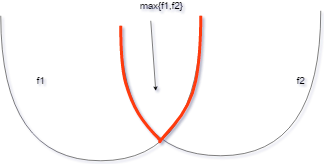
\includegraphics[]{1_3}
\item Composition with linear map.\\
$f \in cvx \R^n$, $A:\R^n \to \R^m$ is a linear map.
$f \circ A (x) = f(Ax) \in cvx \R^n$\\
\begin{align*}
f \circ A (x) & = f(A(\alpha x + (1-\alpha) y)) \\
& = f(A \alpha x + (1-\alpha) A y) \\
& \le \alpha f(Ax) + (a - \alpha) f(Ay)
\end{align*}
\end{itemize}

%---------------------------------------------------------------------------------------
%	CHAPTER 3
%----------------------------------------------------------------------------------------

\chapter{Nonlinear Problem}
Les sujets de ce chapitre sont du néanmoins axées sur des questions
ou l'approche mathématique et physique et demandé 

\section{Équation différentielle}
Sans aucun doute 
\section{Chaos}\index{Mouvement d'un pendule}
Prenons une pause dans l'apprentissage de nouvelles techniques et algorithmes informatiques
pour un peu, et passer du temps en utilisant ce que nous avons appris jusqu'à présent pour enquêter sur quelque chose d'intéressant. Nous allons commencer avec quelque chose de familier: le simple pendule.
\subsection{Pendule simple}
Le pendule simple figure
\subsection{Pendule à deux bras}
\subsection{Mouvements d’un robot}
Qu'est ce qu'il faut savoir quand en veut modélisé le comportement
d'un robot?. Et bien la réponse est tout simplement des mathématiques

\section{Solution non linéaire d'équation algébrique}\index{Solving Nonlinear Algebraic Equations}

Qu'est ce que non-linéaire et qu'est ce que une \'equation alg\'ebrique

Une \'equation alg\'ebrique est un polyn\^ome de la forme $P(x)$

\begin{equation}
\exp(-x)\sin(x) = \cos(x)
\end{equation}

\section{Transport optimal}
C'est quoi le \textit{ transport optimal}?, exemple simple..., le domaine du transport optimal
est très 
%-------------------------------------------------
\section{Le calcul des variations}

\section{Figure}\index{Figure}

\begin{table}[h]
\centering
\begin{tabular}{l l l}
\toprule
\textbf{Treatments} & \textbf{Response 1} & \textbf{Response 2}\\
\midrule
Treatment 1 & 0.0003262 & 0.562 \\
Treatment 2 & 0.0015681 & 0.910 \\
Treatment 3 & 0.0009271 & 0.296 \\
\bottomrule
\end{tabular}
\caption{Table caption}
\end{table}

%
%\begin{figure}[h]
%\centering\includegraphics[scale=0.5]
%\caption{Figure caption}
%\end{figure}

%----------------------------------------------------------------------------------------
%	Technique Avancée
%----------------------------------------------------------------------------------------

\chapter{Outils avancée}

\section{Programmation Orientée Objet}\index{Notations}
\section{D\'ecorateurs}
Les d\'ecorateurs un m\'ecanisme incontournable pour \'ecrire de tr\'es bon code et purement lisible et
portable
\subsection{Optimisation du code}
%\subsection{Cython}
Cython (http://www.cython.org/ ) est un métalangage qui permet de combiner du code
Python et des types de donn\'ees C, pour concevoir des extensions compilables pour
Python.
Dans un module Cython, il est possible de définir des variables C directement dans
le code Python et de définir des fonctions C qui prennent en paramètre des
variables C ou des objets Python.
Cython contr\^ole ensuite de manière transparente la génération de l’extension C, en
transformant le module en code C par le biais des API C de Python.
Toutes les fonctions Python du module sont alors automatiquement publiées.
Le gain de temps dans la conception introduit par Cython est considérable : toute la
mécanique habituellement mise en œuvre pour créer un module d’extension est
entièrement gérée par Cython.
Ainsi, la fonction max() du module calculs.c pr\'ec\'edemment présent\'ee devient :

Les fichiers Cython ont par convention l’extension pyx, en référence à l’ancien nom.

setup.py pour calculs.pyx

\begin{python}
from distutils.core import setup
from distutils.extension import Extension
from Cython.Distutils import build_ext

extension = Extension("calculs", ["calculs.pyx"])

setup(name="calculs", ext_modules=[extension],cmdclass={'build_ext': build_ext})

\end{python}

\subsection{Theano}
Theano est une biblioth\'eque pour l'acc\e'ration du code lent en Python, tr\'es importante et intéressante
elle offre une syntaxe très particulière.
\section{Interface graphique}
Quelle bibliothèque choisir: sous Python en \`a le choix entre diff\'erente, Tkinter, Gtk, Qt, wx et ftk
et il existe encore d'autre bibliothques qui sont con\c{c}u pour le calcul et application scientifique
\'editer par Thought[...] dans cette section nous allons  
\subsection{PyQt}


\end{document}